% =========================================================================
% LaTeX TEMPLATE FOR GEM5 BRANCH PREDICTION ASSIGNMENT
% =========================================================================
% This template is designed to meet the requirements outlined in the
% assignment PDF. Fill in the sections with your own content.
%
% To compile this document, you will need a LaTeX distribution (like MiKTeX,
% TeX Live, or MacTeX) and a LaTeX editor (like TeXstudio, VS Code with

% LaTeX Workshop, or Overleaf).
% =========================================================================

\documentclass[11pt, a4paper]{article}

% --- PACKAGE IMPORTS ---
\usepackage[margin=1in]{geometry} % For setting page margins
\usepackage{graphicx}             % For including images/plots
\usepackage{amsmath}              % For advanced math typography
\usepackage{booktabs}             % For professional-quality tables
\usepackage{hyperref}             % For clickable links and references
\usepackage{listings}             % For formatting code snippets
\usepackage{xcolor}               % For defining colors

% --- HYPERREF SETUP ---
\hypersetup{
    colorlinks=true,
    linkcolor=blue,
    filecolor=magenta,
    urlcolor=cyan,
    pdftitle={Evaluating Branch Prediction Schemes},
    pdfpagemode=FullScreen,
}

% --- LISTINGS (CODE) SETUP ---
\definecolor{codegreen}{rgb}{0,0.6,0}
\definecolor{codegray}{rgb}{0.5,0.5,0.5}
\definecolor{codepurple}{rgb}{0.58,0,0.82}
\definecolor{backcolour}{rgb}{0.95,0.95,0.92}

\lstdefinestyle{mystyle}{
    backgroundcolor=\color{backcolour},
    commentstyle=\color{codegreen},
    keywordstyle=\color{magenta},
    numberstyle=\tiny\color{codegray},
    stringstyle=\color{codepurple},
    basicstyle=\ttfamily\footnotesize,
    breakatwhitespace=false,
    breaklines=true,
    captionpos=b,
    keepspaces=true,
    numbers=left,
    numbersep=5pt,
    showspaces=false,
    showstringspaces=false,
    showtabs=false,
    tabsize=2
}
\lstset{style=mystyle}

% =========================================================================
% --- DOCUMENT START ---
% =========================================================================
\begin{document}

% --- TITLE PAGE ---
\title{
    \textbf{Evaluating Branch Prediction Schemes with an Out-of-Order Core in gem5} \\
    \vspace{0.5cm}
    \large Architecture for High Performance Computers / COL718
}
\author{
    Arpit Prasad (2022EE11837) \\
    \texttt{ee1221837@iitd.ac.in}
    \and
    Devansh Panday (2022EE31583) \\
    \texttt{ee3221583@iitd.ac.in}
}
\date{\today}
\maketitle
\thispagestyle{empty} % No page number on the title page
\newpage

% --- GROUP CONTRIBUTIONS ---
\section{Group Contributions}
% As per deliverable #6, clearly identify the contributions of each partner.
% Be specific.
% Example:
\begin{itemize}
    \item \textbf{Arpit Prasad}
    \begin{itemize}
        \item Extracted Results
        \item Produced Report and Slides
    \end{itemize}
    \item \textbf{Devansh Panday}
    \begin{itemize}
        \item Configured all the Predictor.
    \end{itemize}
\end{itemize}

% --- MACHINE CONFIGURATION ---
\section{Machine Configuration}
% As per deliverable #7, provide the configuration of the machine used for
% generating data. On Linux, you can get this from /proc/cpuinfo, /proc/meminfo, etc.
% Or use a command like `lscpu`.
% Example:
\begin{itemize}
    \item \textbf{CPU:} Intel(R) Core(TM) i5-1340P @ 3.70GHz
    \item \textbf{Cores:} 6 (12 threads)
    \item \textbf{L1d/L1i/L2/L3 Cache:} 448KiB / 640KiB / 9MiB / 12MiB
    \item \textbf{Memory:} 32 GB DDR4 @ 3200MHz
    \item \textbf{OS:} Ubuntu 22.04.1 LTS
    \item \textbf{gem5 Version:} [Specify the version or commit hash you used]
\end{itemize}

% --- BACKGROUND AND HYPOTHESIS ---
\section{Background and Hypothesis}
\subsection{Background}
% Introduce the concept of branch prediction in modern out-of-order processors.
% Explain why it is critical for performance. Briefly describe the different
% classes of predictors you are evaluating (e.g., static vs. dynamic,
% one-level vs. two-level, hybrid).
Branch Prediction is a technique widely used to increase the IPC for modern day OOO Processors. The instructions to execute are fetched in blocks, however if one of the instruction turns out to be a branch, we face loss of IPC, since we would have to drop all the instructions ahead of that branch in the block of instrcution and fetch new intstruciton following after the Traget Branch.

\subsection{Hypothesis}

We hypothesize that more complex predictors like Tournament and
Perceptron will significantly outperform simpler schemes like Bimodal,
especially on the branch-heavy workload, leading to higher IPC. For the
compute-heavy workload, we expect the difference in performance to be less
pronounced, as branch mispredictions are a smaller bottleneck.


% --- EXPERIMENT METHODOLOGY ---
\section{Experiment Methodology}
\subsection{Microarchitectural Parameters}
The following parameters were kept constant across various iterations of the experiment:
\begin{enumerate}
    \item Simulator: gem5 (version)
    \item CPU Model: DerivO3CPU
    \item ISA: X86
    \item OOO core parameters 
    \begin{enumerate}
        \item ROB Size: 192 Instructions
        \item IQ entries: 64 Instructions
        \item Fetch Width: 4 Instructions
        \item Issue Width: 4 Instructions
    \end{enumerate}
\end{enumerate}

\subsection{Branch Predictors Evaluated}
% List and briefly describe the configuration of each predictor you tested.
% Mention key parameters like table sizes, history lengths, counter bits, etc.
% e.g., Bimodal (4096 entries, 2-bit counters), Gshare (12-bit global history,
% 8192 entries), etc.
The following are the list of Branch Predictors that were used for Evaluation:

\begin{enumerate}
    \item \textbf{BiModalBP} - This is a simple hardware level branch prediction mechnanism that uses two bit saturating counter to determine the surity of a branch prediction from previous prediction results
    \item \textbf{GShareBP} - This is a dynamic Branch Predictor that takes into account for the Global History of Branch predictors along with the current program counter and makes prediction on the branch type
    \item \textbf{LocalBP} - Similar to GShareBP, but uses a Local History Table instead of globally maintaining the last branch predictions
    \item MultiperspectivePerceptron - 
    \item \textbf{TournamentBP}
\end{enumerate}

\subsection{Workloads}
% Describe the workloads you chose. Justify your choices, explaining which one is
% branch-heavy and which is compute-heavy. Mention the specific inputs used for each.
% (e.g., MiBench/susan, PARSEC/blackscholes)
The following table tabulates the workloads that were experimented with and short description of why they are categorized either as Branch Heavy or Compute Heavy

\begin{table}[h!]
    \centering
    \caption{Workloads}
    \begin{tabular}{|c|c|c|c|}
        \hline
        \textbf{Sl. No.} & \textbf{Workload} & \textbf{Branch or Compute Heavy} & \textbf{Short Reason} \\
        \hline
        1 & BasicMath & Compute Heavy & Lots of calulations \\
        \hline
        2 & QuickSort & Branch Heavy & Many checks for Comparisions \\
        \hline
    \end{tabular}
\end{table}

\subsection{Data Collection}
% Explain how you ran the experiments to ensure fair comparison.
% - Warmup strategy (e.g., fast-forwarding, checkpoints).
% - Region of Interest (ROI): How many instructions were simulated for stats collection?
% - Repetitions: Did you run each experiment multiple times to check for variance?

The following are some key information in regards to the data collection process 
\begin{enumerate}
    \item Warmup strategy: The offset for Instructions was 2M for fast forwarding and 100M for checkpoints.
    \item Region of Interest
    \item Repetitions: The code was run three times to observer the variability of metrics across runs
\end{enumerate}

% --- RESULTS ---
\section{Results}
% Present your collected data clearly using tables and figures.
% Do not interpret the results here; just present them.

\subsection{Summary Data}
% Use a table to present the primary metrics for each workload and predictor combination.
% This directly corresponds to task 6.1 in the assignment.
\begin{table}[h!]
    \centering
    \caption{Performance Metrics for the \textit{Branch-Heavy Workload}}
    \label{tab:branch_heavy_results}
    \begin{tabular}{l c c c}
        \toprule
        Predictor         & IPC   & Misprediction Rate (\%) & Recovery Penalty (Cycles) \\ \midrule
        Baseline          & 0.42  & 0.00                    & 20.0                      \\
        BiModeBP          & 0.42  & 3.35                    & 20.0                      \\
        GShareBP          & 0.42  & 27.56                   & 20.0                      \\
        LocalBP           & 0.42  & 5.16                    & 20.0                      \\
        MultiperspectivePerceptron8KB & 0.42  & 2.69                    & 20.0                      \\
        TournamentBP      & 0.42  & 3.02                    & 20.0                      \\
        \bottomrule
    \end{tabular}
    \\ \vspace{0.5cm} % Add some space between tables
    \caption{Performance Metrics for the \textit{Compute-Heavy Workload}}
    \label{tab:compute_heavy_results}
    \begin{tabular}{l c c c}
        \toprule
        Predictor         & IPC   & Misprediction Rate (\%) & Recovery Penalty (Cycles) \\ \midrule
        Baseline          & 0.45  & 0.00                    & 20.0                      \\
        BiModeBP          & 0.45  & 2.04                    & 20.0                      \\
        GShareBP          & 0.45  & 31.60                   & 20.0                      \\
        LocalBP           & 0.45  & 3.99                    & 20.0                      \\
        MultiperspectivePerceptron8KB & 0.45  & 0.87                    & 20.0                      \\
        TournamentBP      & 0.45  & 1.41                    & 20.0                      \\
        \bottomrule
    \end{tabular}
    % ... Create a similar table for the compute-heavy workload ...
\end{table}

\subsection{Graphical Analysis}
% Use plots to visualize the results, as requested in task 6.2.
% Make sure your plots are clearly labeled with a title, axis labels, and a legend.

\begin{figure}[h!]
    \centering
    % Replace 'ipc_plot.png' with the filename of your generated plot.
    % It's good practice to store image files in a subfolder, e.g., 'images/'.
    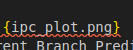
\includegraphics[width=0.8\textwidth]{/home/arpit/Desktop/iitd/sem_7/COL718/projects/Branch-Predictor-Test/img/ipc_plot.png}
    \caption{IPC Comparison Across Different Branch Predictors for Each Workload.}
    \label{fig:ipc_chart}
\end{figure}

\begin{figure}[h!]
    \centering
    % Create a scatter plot of misprediction rate vs. IPC.
    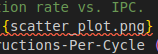
\includegraphics[width=0.8\textwidth]{/home/arpit/Desktop/iitd/sem_7/COL718/projects/Branch-Predictor-Test/img/scatter_plot.png}
    \caption{Misprediction Rate vs. Instructions-Per-Cycle (IPC).}
    \label{fig:scatter_plot}
\end{figure}
\clearpage % Helps with figure placement

% --- ANALYSIS AND DISCUSSION ---
\section{Analysis and Discussion}
% This is the most important section. Interpret your results and explain *why*
% they look the way they do. Refer back to your tables and figures.
% Address the questions from task 6.3:
% - Which predictor performed best overall and why?
% - Discuss the performance of different predictors on different workloads.
% - How do predictor improvements translate (or not) into IPC improvements?
%   (e.g., is the pipeline bottlenecked elsewhere?)
% - Discuss any interesting or unexpected results.
% - If you tested the perceptron predictor, how did it compare?
% - Comment on variability across runs if you performed multiple runs.

% --- CONCLUSION AND LIMITATIONS ---
\section{Conclusion and Limitations}
\subsection{Conclusion}
% Summarize the key findings of your study. Revisit your initial hypothesis
% and state whether your results supported it.

\subsection{Limitations}
% Discuss the limitations of your work.
% - What aspects were not covered? (e.g., power consumption, hardware cost).
% - Were the chosen workloads representative of all possible applications?
% - Are there any limitations of the gem5 model itself?
% - What could be done in future work to build upon your findings?

% --- REFERENCES ---
% Use this section if you cite any external papers, books, or resources.
\begin{thebibliography}{9}
    \bibitem{gem5}
    The gem5 Simulator System.
    \url{http://www.gem5.org}

    \bibitem{yeh_patt}
    T-Y. Yeh and Y. N. Patt,
    "Two-Level Adaptive Branch Prediction,"
    \textit{in Proceedings of the 24th ACM/IEEE Annual International Symposium on Microarchitecture}, 1991.

\end{thebibliography}

% --- APPENDIX ---
\appendix
\section{Run Script Example}
% It can be helpful to include an example of your run scripts or important
% code snippets in an appendix.
% \begin{lstlisting}[language=Bash, caption={Example gem5 run script for GShareBP.}, label={lst:run_script}]
% #!/bin/bash
% build/X86/gem5.opt configs/example/se.py \
%   --cpu-type=DerivO3CPU \
%   --caches --l2cache \
%   --bp-type=GShareBP \
%   --gshare-history=12 \
%   --gshare-table-size=8192 \
%   --cmd=/path/to/workload \
%   --options="input args" \
%   --maxinsts=100000000
% \end{lstlisting}

\end{document}
% =========================================================================
% --- DOCUMENT END ---
% =========================================================================

